%!TEX TS-program = XeLaTeX
%!TEX TS-program = XeLaTeX
\documentclass[11pt]{article}

\usepackage{amssymb}
\usepackage{amsthm}
\usepackage{amsmath}
\usepackage{mathtools}

\usepackage{fancyhdr}
\usepackage{graphicx}
\usepackage[top=3cm, left=2cm, right=2cm, headheight = 90pt]{geometry}
\usepackage{xltxtra}
\usepackage[font=small,labelfont=bf]{caption}

\usepackage{multicol}

\renewcommand{\theenumi}{\alph{enumi}}


\def\leq{\leqslant}
\def\geq{\geqslant}
\def\N{\mathbb N}
\def\R{\mathbb R}
\def\Z{\mathbb Z}
\DeclarePairedDelimiter\set\{\}

\def\prob{}

\theoremstyle{definition}
\newtheorem{problem}{\prob}


\pagestyle{fancy}

%%!TEX TS-program = XeLaTeX

\fancyfoot[CE,CO]{}  % this is to remove page numbers (as you might want for single page docs)

%%!TEX TS-program = XeLaTeX
\renewcommand{\figurename}{Attēls}

\fancyhead[C]{{\Large\bf Graphs 3 - Solutions}\\ \date}

\renewcommand{\theenumi}{\alph{enumi}}

\begin{document}

\noindent
 
\filbreak

%1
\begin{problem}
\textit{[BW1994PL19]}


\textbf{Problem}

The Wonder Island Intelligence Service has $16$ spies in Tartu. Each of them watches on some of his colleagues. It is known that if spy $A$ watches on spy $B$, then $B$ does not watch on $A$. Moreover, any $10$ spies can numbered in such a way that the first spy watches on the second, the second watches on the third, $ \dots $, the tenth watches on the first. 

Prove that any $11$ spies can also be numbered is a similar manner!


\textbf{Solution - Double counting, two level proof from opposite}

We call spies $A$ and $B$ \textit{neutral} to each other if neither $A$ watches $B$ nor $B$ watches $A$. For each spy $A_1$ denote $a_1$, $b_1$ and $c_1$ the number of spies that watches on $A_i$, the number of spies $A_i$ watches and the number of spies neutral to $A_i$. Clearly we have
$$
a_i+b_i+c_i = 15
$$
And, we have 
$$
a_i+c_i \le 8
$$
$$
b_i+c_i \le 8
$$
because if any of the these two inequalities did not hold, we could select $10$ spies that could not be cyclically watching each other. Adding together these inequalities and equality we get that $c_i \le 1$, that means that for any $A_i$ number of spies neutral to $A_i$ is $0$ or $1$

Now suppose the opposite, that there is a a group of $11$ spies that cannot be numbered as required. Let $B$ be an arbitrary spy in this group. Name other $10$ spies in this group $C_1, C_2, \dots, C_{10}$ so that $C_1$ watches $C_2, \dots, C_{10}$ watches $C_1$. Suppose, that none of these $C_1, \dots, C_{10}$ is neutral to $B$. Some of the spies from $C$ group must watch $B$ (because $b_B \le 8$), and as it is cyclical, say $C_1$ watches $B$. 

Can $B$ watch $C_2$? No, because then we could insert $B$ into the cycle, between $C_1$ and $C_2$ and get a cycle with $11$ spies, which we assumed does not exist. So $C_2$ must also watch $B$. But by the same argument, $C_3$ must watch $B$, $C_4$ must watch $B$, $\dots$, $C_{10}$ must watch $B$. Which is impossible, since $a_B \le 8$. 

Therefore one of our assumptions must be false. First assume, that assumption of not having neutrals among $C_i$ is false, but that is equivalent to saying that between any $11$ spies each must have exactly one neutral, which is impossible by parity of vertex powers (you have to imagine "neutral" as another kind of edges to see it).

Therefore our second assumption - that there are such $11$ spies that cannot be ordered in a cycle, exist - is false, and any $11$ can be ordered in a cycle.
\end{problem}
%

\filbreak

%2
\begin{problem}
\textit{[BW2010PL7]}



\textbf{Problem}


There are some cities in a country; one of them is the capital. For any two cities $A$ and $B$ there is a direct flight from $A$ to $B$ and a direct flight from $B$ to $A$, both having the
same price. Suppose that all round trips with exactly one landing in every city have the same total cost. 

Prove that all round trips that miss the capital and with exactly one landing in every remaining city cost the same!



\textbf{Solution - combinatorial vs algebraic proof}


Let $C$ be the capital and $C_1, C_2, \dots, C_n$ be the remaining cities. Denote by $d(x, y)$
the price of the connection between the cities $x$ and $y$, and let $\sigma$ be the total price of a round
trip going exactly once through each city.


Now consider a particular round trip missing the capital and visiting every other city exactly once; let $s$ be the total price of that trip. Suppose $C_i$ and $C_j$ are two consecutive cities on the route.
Replacing the flight $C_i \rightarrow C_j$ by two flights: from $C_i$ to the capital and from the capital to $C_j$, we
get a round trip through all cities, with total price $\sigma$. It follows that $\sigma = s+d(C, C_i)+d(C, C_j )−d(C_i, C_j )$, so it remains to show that the quantity $\alpha(i,j) = d(C, C_i) + d(C, C_j )−d(C_i, C_j )$ is the same for all 2-element subsets $\set{i, j} \in \set{1, 2, . . . , n}$.



For this purpose, note that $\alpha(i, j) = \alpha(i, k)$ whenever $i, j, k$ are three distinct indices; indeed,
this equality is equivalent to $d(C_j , C) + d(C, C_i) + d(C_i, C_k) = d(C_j , C_i) + d(C_i, C) + d(C, C_k)$, which is true by considering any trip from $C_k$ to $C_j$ going through all cities except $C$ and $C_i$ exactly once and completing this trip to a round trip in two ways: $C_j \rightarrow C \rightarrow C_i \rightarrow C_k$ and $C_j \rightarrow C_i \rightarrow C \rightarrow C_k$. Therefore the values of $\alpha$ coincide on any pair of 2-element sets sharing a common element. 

But then clearly $\alpha(i, j) = \alpha(i, j^\prime)= \alpha(i^\prime, j^\prime)$ for all indices $i, j, i^\prime, j^\prime$ with $i\ne j, i^\prime \ne j^\prime $, and the solution is complete.

\end{problem}
%
\filbreak
%3
\begin{problem}
\textit{[IMO2007PL3]}

\textbf{Problem}

In a mathematical competition some competitors are friends. Friendship is always mutual. Call a group of competitors a \textit{clique} if each two of them are friends. (In particular, any group of fewer than two competitors is a clique.) The number of members of a clique is called its size. 

Given that, in this competition, the largest size of a clique is even, prove that the competitors can be arranged in two rooms such that the largest size of a clique contained in one room is the same as the largest size of a clique contained in the other room!

\textbf{Solution - Algorithmic solution}

We present an algorithm to arrange the competitors. Let the rooms be $A$ and $B$. We start with an
initial arrangement, and then we modify it several times by sending one person to the other room. At
any state of the algorithm, $A$ and $B$ denote the sets of the competitors in the rooms, and $c(A)$ and
$c(B)$ denote the largest sizes of cliques in the rooms.

\textbf{STEP 1:} Let $M$ be one of the cliques of largest size, $\abs{M} = 2m$. Send all members of $M$ to $A$ and all
others to $B$.  

Since $M$ is a clique of the largest size, we have $c(A) = \abs{M} \geq  c(B)$.

\textbf{STEP 2:} While $c(A) > c(B)$, send one person from $A$ to $B$.
Note that $c(A) > c(B)$ implies that $A$ is not empty. In each step, $c(A)$ decreases by $1$ and $c(B)$
increases by at most $1$. So at the end we have $c(A) \leq c(B) \leq c(A) + 1$.
We also have $c(A) = \abs{A}\geq m$ at the end. Otherwise we would have at least $m + 1$ members of $M$ in
$B$ and at most $m − 1$ in $A$, implying $c(B) − c(A) \geq (m + 1) − (m − 1) = 2$.


\textbf{STEP 3:}  Let $k = c(A)$. If $c(B) = k$ then STOP.
If we reached $c(A) = c(B) = k$ then we have found the desired arrangement. In all other cases we have
$c(B) = k + 1$. From the estimate above we also know that $k = \abs{A} = \abs{A \cap  M} \geq m$ and $\abs{B \cap M} \leq m$.


\textbf{STEP 4:} If there exists a competitor $x \in B \cap M$ and a clique $C \subset B$ such that $\abs{C} = k + 1$ and $x \notin C$,
then move $x$ to $A$ and STOP.
After moving $x$ back to $A$, we will have $k + 1$ members of $M$ in $A$, thus $c(A) = k + 1$. Due to $x \notin C$,
$c(B) = \abs{C}$ is not decreased, and after this step we have $c(A) = c(B) = k + 1$.
If there is no such competitor $x$, then in $B$ all cliques of size $k + 1$ contain $B \cap M$ as a subset.


\textbf{STEP 5:} While $c(B) = k + 1$, choose a clique $C\subset B$ such that $\abs{C} = k + 1$ and move one member of
$C \setminus M$ to $A$.
Note that $\abs{C} = k + 1 > m \geq  \abs{B \cap M}$, so $C \setminus M$ is not empty. Every time we move a single person
from $B$ to $A$, $c(B)$ decreases by at most $1$. Hence, at the end of this loop we have $c(B) = k$.
In $A$ we have the clique $A \cap M$ with size $\abs{A \cap M} = k$, thus $c(A) \geq k$. We prove that there is no clique
of larger size there. Let $Q \subset A$ be an arbitrary clique. We show that $\abs{Q}  \leq  k$.
In $A$, specially in set $Q$, there can be two types of competitors: 
\begin{itemize}
\item (i) some members of $M$. Since $M$ is a clique, they are friends with all members of $B \cap M$; 
\item (ii) competitors which were moved to $A$ in STEP 5. Each of them has been in a clique with $B \cap M$ so they are also friends with all members of $B \cap M$.
\end{itemize}
Hence all members of $Q$ are friends with all the members of $B \cap M$. Sets $Q$ and $B \cap M$ are cliques
themselves, so $Q \cup (B \cap M)$ is also a clique. Since $M$ is a clique of the largest size, 
$$\abs{M}  \geq \abs{Q \cup (B \cap M)} = \abs{Q} + \abs{B \cap M} = \abs{Q} + \abs{M} − \abs{A \cap M}, i.e. \abs{Q} \leq \abs{A \cap M} = k. $$ 
Finally after STEP 5 we have $c(A) = c(B) = k$.


\end{problem}
%
\filbreak
%4
\begin{problem}

\textit{[IMO2013SLC3]}


\textbf{Problem}


A crazy physicist discovered a new kind of particle which he called an \textit{imon}, after some of them mysteriously appeared in his lab. Some pairs of imons in the lab can be entangled, and each imon can participate in many entanglement relations. The physicist has found a way to perform the following two kinds of operations with these particles, one operation at a time.
\begin{enumerate}
\item \label{op1}  If some imon is entangled with an odd number of other imons in the lab, then the physicist
can destroy it.
\item \label{op2}  At any moment, he may double the whole family of imons in his lab by creating a copy $I^\prime$ of each imon $I$. During this procedure, the two copies $I^\prime$ and $J^\prime$ become entangled if and only if the original imons $I$ and $J$ are entangled, and each copy $I^\prime$ becomes entangled with its original imon $I$; no other entanglements occur or disappear at this moment.
\end{enumerate}
Prove that the physicist may apply a sequence of such operations resulting in a family of imons, no two of which are entangled!


\textbf{Solution - Proper coloring}


Let us consider a graph with the imons as vertices, and two imons being connected if and only if they are entangled. \textit{Proper coloring} of a graph $G$ is a coloring of its vertices in several colors so that every two connected vertices have different colors. 

\begin{lemma}
Assume that a graph $G$ admits a proper coloring in $n$ colors $(n > 1)$. Then one may perform a sequence of operations a. and b. resulting in a graph which admits a proper coloring in $n - 1$ colors.
\end{lemma}

\begin{proof}
Let us apply repeatedly operation \textbf{\ref{op1}.} to any appropriate vertices while it is possible. Since the number of vertices decreases, this process finally results in a graph where all the degrees are even. Surely this graph also admits a proper coloring in $n$ colors $1,\dots, n$; let us fix this coloring.


Now apply the operation \textbf{\ref{op2}.} to this graph. A proper coloring of the resulting graph in $n$ colors still exists: one may preserve the colors of the original vertices and color the vertex $I^\prime$ in a color $k+1 (mod \  n)$ if the vertex $I$ has color $k$. Then two connected original vertices still have different colors, and so do their two connected copies. On the other hand, the vertices $I$ and $I^\prime$ have different colors since $n > 1$.

All the degrees of the vertices in the resulting graph are odd, so one may apply operation \textbf{\ref{op1}.} to delete consecutively all the vertices of color $k$ one by one; no two of them are connected by an edge, so their degrees do not change during the process. Thus, we obtain a graph admitting a proper coloring in $n - 1$ colors, as required. The lemma is proved. 
\end{proof}

Now, assume that a graph $G$ has $n$ vertices; then it admits a proper coloring in $n$ colors. Applying repeatedly the lemma we finally obtain a graph admitting a proper coloring in one color, that is -- a graph with no edges, as required.
\end{problem}
%
\filbreak
%5
\begin{problem}
\textit{[IMO2015SLC7]}

\textbf{Problem}


In a company of people some pairs are enemies. A group of people is called \textit{unsociable} if the number of members in the group is odd and at least $3$, and it is possible to arrange all its members around a round table so that every two neighbors are enemies. 

Given that there are at most $2015$ unsociable groups, prove that it is possible to partition the company into $11$ parts so that no two enemies are in the same part!

\textbf{Solution - Proper coloring, Chromatic number, number of odd-sized subsets}

Let $G = (V, E)$ be a graph where $V$ is the set of people in the company and $E$ is the set of the enemy pairs — the edges of the graph. In this language, partitioning into $11$ disjoint enemy-free subsets means properly coloring the vertices of this graph with $11$ colors. We will prove the following more general statement.

\begin{claim} Let $G$ be a graph with chromatic number $k \geq  3$. Then $G$ contains at least $2^{k-1} - k$ unsociable groups.
\end{claim}

\textit{Chromatic number} of $G$ is the least $k$ such that a proper coloring 
\begin{equation}
\label{propcoloring}
V = V_1 \sqcup \dots \sqcup V_k
\end{equation}
exists. In view of $2^{11} - 12 > 2015$, the claim implies the problem statement. 

Let $G$ be a graph with chromatic number $k$. We say that a proper coloring (\ref{propcoloring}) of $G$ is \textit{leximinimal}, if the $k$-tuple $(\abs{V_1}, \abs{V_2}, \dots , \abs{V_k})$ is lexicographically minimal; in other words, the following conditions are satisfied: 
\begin{itemize}
\item the number $n_1 = \abs{V_1}$ is minimal; 
\item the number $n_2 = \abs{V_2}$ is
minimal, subject to the previously chosen value of $n_1$; 
\item \dots  
\item the number $n_{k-1}  = \abs{V_{k-1}}$ is minimal,
subject to the previously chosen values of $n_1, \dots , n_{k-2}$.
\end{itemize}
The following lemma is the core of the proof.
\begin{lemma}
\label{leximinlemma} 
Suppose that $G = (V, E)$ is a graph with odd chromatic number $k \ge 3$, and let (\ref{propcoloring}) be one of its leximinimal colorings. Then $G$ contains an odd cycle which visits all color classes
$V_1, V_2, \dots, V_k$.
\end{lemma}
\begin{proof}
Let us call a cycle colorful if it visits all color classes. 

Due to the definition of the chromatic number, $V_1$ is nonempty. Choose an arbitrary vertex $v \in V_1$. We will construct a colorful odd cycle that has only one vertex in $V_1$, and this vertex is $v$. 

We draw a subgraph of $G$ as follows. Place $v$ in the center, and arrange the sets $V_2, V_3, \dots , V_k$ in counterclockwise circular order around it. For convenience, let $V_{k+1} = V_2$. We will draw arrows to add direction to some edges of $G$, and mark the vertices these arrows point to. First we draw arrows from $v$ to all its neighbors in $V_2$, and mark all those neighbors. If some vertex $u \in V_i$ with $i \in {2, 3, \dots , k}$ is already marked, we draw arrows from $u$ to all its neighbors in $V_{i+1}$ which are not marked yet, and we mark all of them. We proceed doing this as long as it is possible. The process of marking is exemplified in Figure 1.

Notice that by the rules of our process, in the final state, marked vertices in $V_i$ cannot have unmarked neighbors in $V_{i+1}$. Moreover, $v$ is connected to all marked vertices by directed paths. 

Now move each marked vertex to the next color class in circular order (see an example in Figure 2). In view of the arguments above, the obtained coloring $V_1 \sqcup W_2 \sqcup \dots \sqcup W_k$ is proper. 

Notice that $v$ has to have a neighbor $w \in W_2$, because otherwise
\begin{equation}
(V_1  \setminus \set{v}) \sqcup (W_2 \cup \set{v}) \sqcup W_3 \sqcup \dots \sqcup W_k
\end{equation}
would be a proper coloring lexicographically smaller than (\ref{propcoloring}). If $w$ was unmarked, i.e., $w$ was an element of $V_2$, then it would be marked at the beginning of the process and thus moved to $V_3$, which did not happen. Therefore, $w$ is marked and $w \in V_k$.

\begin{center}
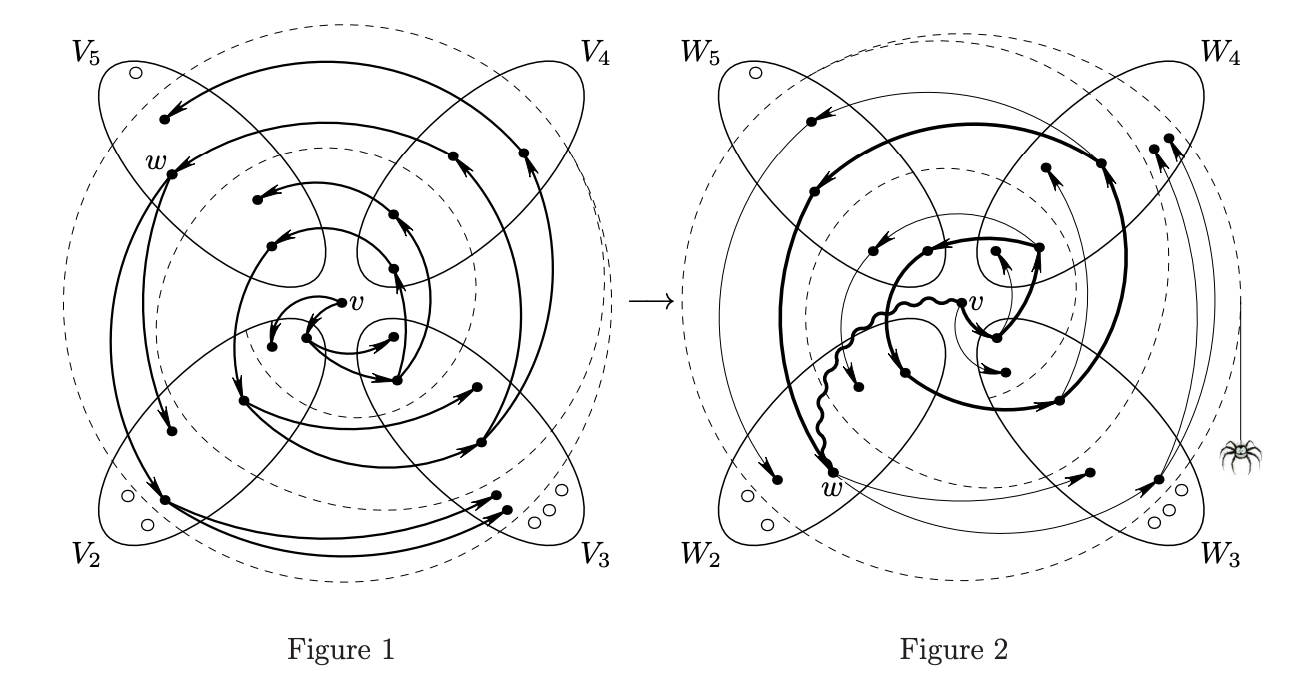
\includegraphics[width=18cm]{spider.png}
%\captionof{figure}{Crossing a narrow bridge}
\label{fig:spider}
\end{center}

Since $w$ is marked, there exists a directed path from $v$ to $w$. This path moves through the sets $V_2, \dots , V_k$ in circular order, so the number of edges in it is divisible by $k - 1$ and thus even.
Closing this path by the edge $w \rightarrow v$, we get a colorful odd cycle, as required.
\end{proof}

Proof of the claim. 
\begin{proof}
Let us choose a leximinimal coloring (\ref{propcoloring}) of $G$. For every set $C \subseteq  \set{1, 2, \dots, k}$ such that $\abs{C}$ is odd and greater than $1$, we will provide an odd cycle visiting exactly those color classes whose indices are listed in the set $C$. This property ensures that we have different cycles for different choices of $C$, and it proves the claim because there are $2^{k-1} - k$ choices for the set C.


Let $V_C = \bigcup_{c \in C}V_c$, and let $G_C$ be the induced subgraph of $G$ on the vertex set $V_C$. We also have the induced coloring of $V_C$ with $\abs{C}$ colors; this coloring is of course proper. Notice further that the induced coloring is leximinimal: if we had a lexicographically smaller coloring  
$(W_c)_{c \in C}$ of $G_C$, then these classes, together the original color classes $V_i$ for $i \notin C$, would provide a proper coloring which is lexicographically smaller than (\ref{propcoloring}). Hence Lemma \ref{leximinlemma}, applied to the subgraph $G_C$ and its leximinimal coloring $(V_c)_{c \in C}$, provides an odd cycle that visits exactly those color classes that are listed in the set $C$. 
\end{proof}
\end{problem}
%
\filbreak
\end{document}
